\section{Diagramma dei casi d'uso}

In figura \ref{fig:use-cases} \`e illustrata una versione ad alto livello del diagramma dei casi d'uso del progetto.

\begin{figure*}
	\centering
	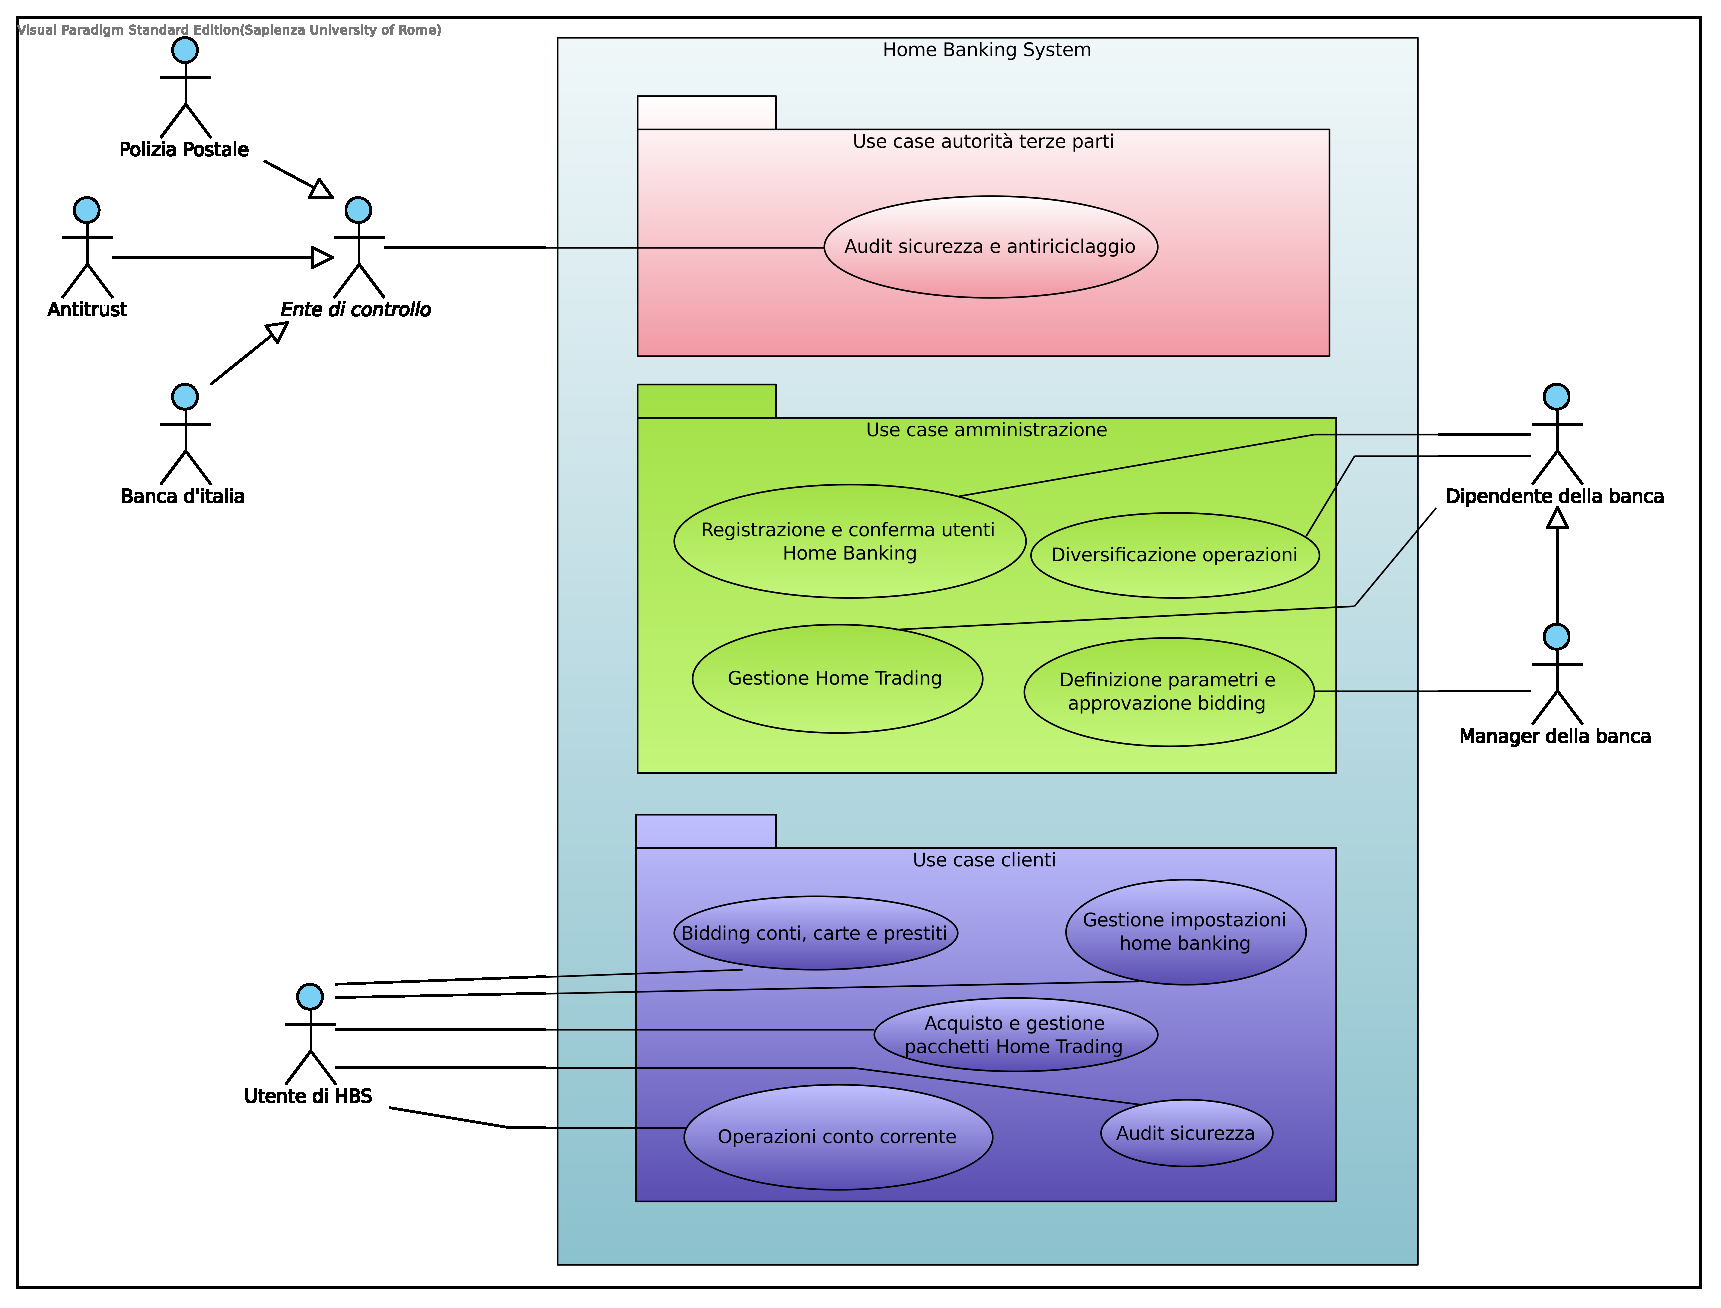
\includegraphics[width=\textwidth]{Images/Home_Banking_inception_use_cases.eps}
	\caption{Attori del sistema di Home Banking e relativi use cases.}
	\label{fig:use-cases}
\end{figure*}

\subsection{Use case di amministrazione}

Di seguito sono illustrati i diagrammi di use case relativi all'amministrazione della banca.

\begin{itemize}
	\item in figura~\ref{fig:use-cases:amministrazione} sono indicati gli use case più alto livello dell'amministrazione;

	\item in figura~\ref{fig:use-cases:amministrazione:gestione-utenti} sono indicati gli use case relativi alla gestione degli account utenti;

	\item in figura~\ref{fig:use-cases:amministrazione:gestione-bidding} sono indicati gli use case relativi alla creazione e alla gestione delle regole di bidding.
	Gli use case comprendono:
	\begin{itemize}
		\item \hyperref[sec:use-case:BIDVIS]{\idBIDVIS};
	\end{itemize}

	\item in figura~\ref{fig:use-cases:amministrazione:gestione-operazioni-veloci} sono indicati gli use case relativi alla creazione e modifica delle operazioni veloci.
\end{itemize}

\begin{figure*}
	\centering
	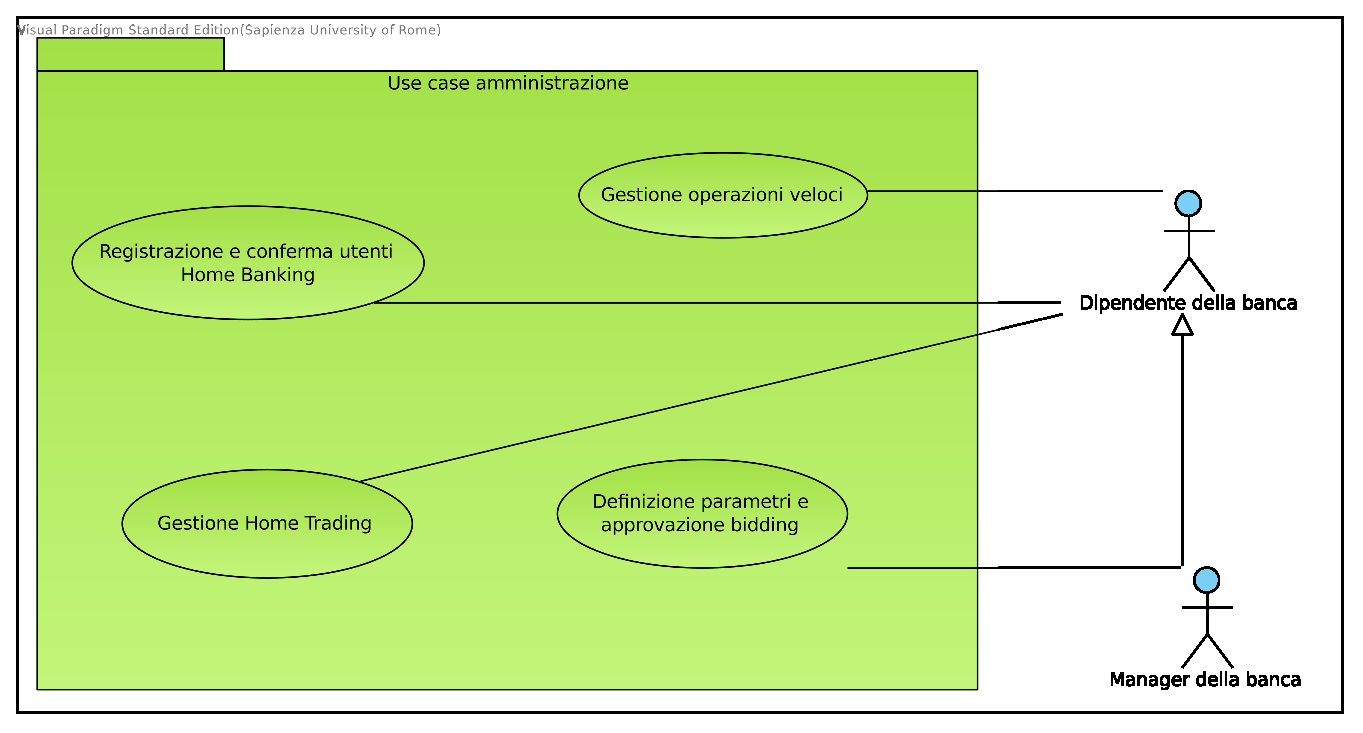
\includegraphics[width=\textwidth]{Images/use-cases/Amministrazione.eps}
	\caption{Diagramma degli use case di amministrazione.}
	\label{fig:use-cases:amministrazione}
\end{figure*}

\begin{figure*}
	\centering
	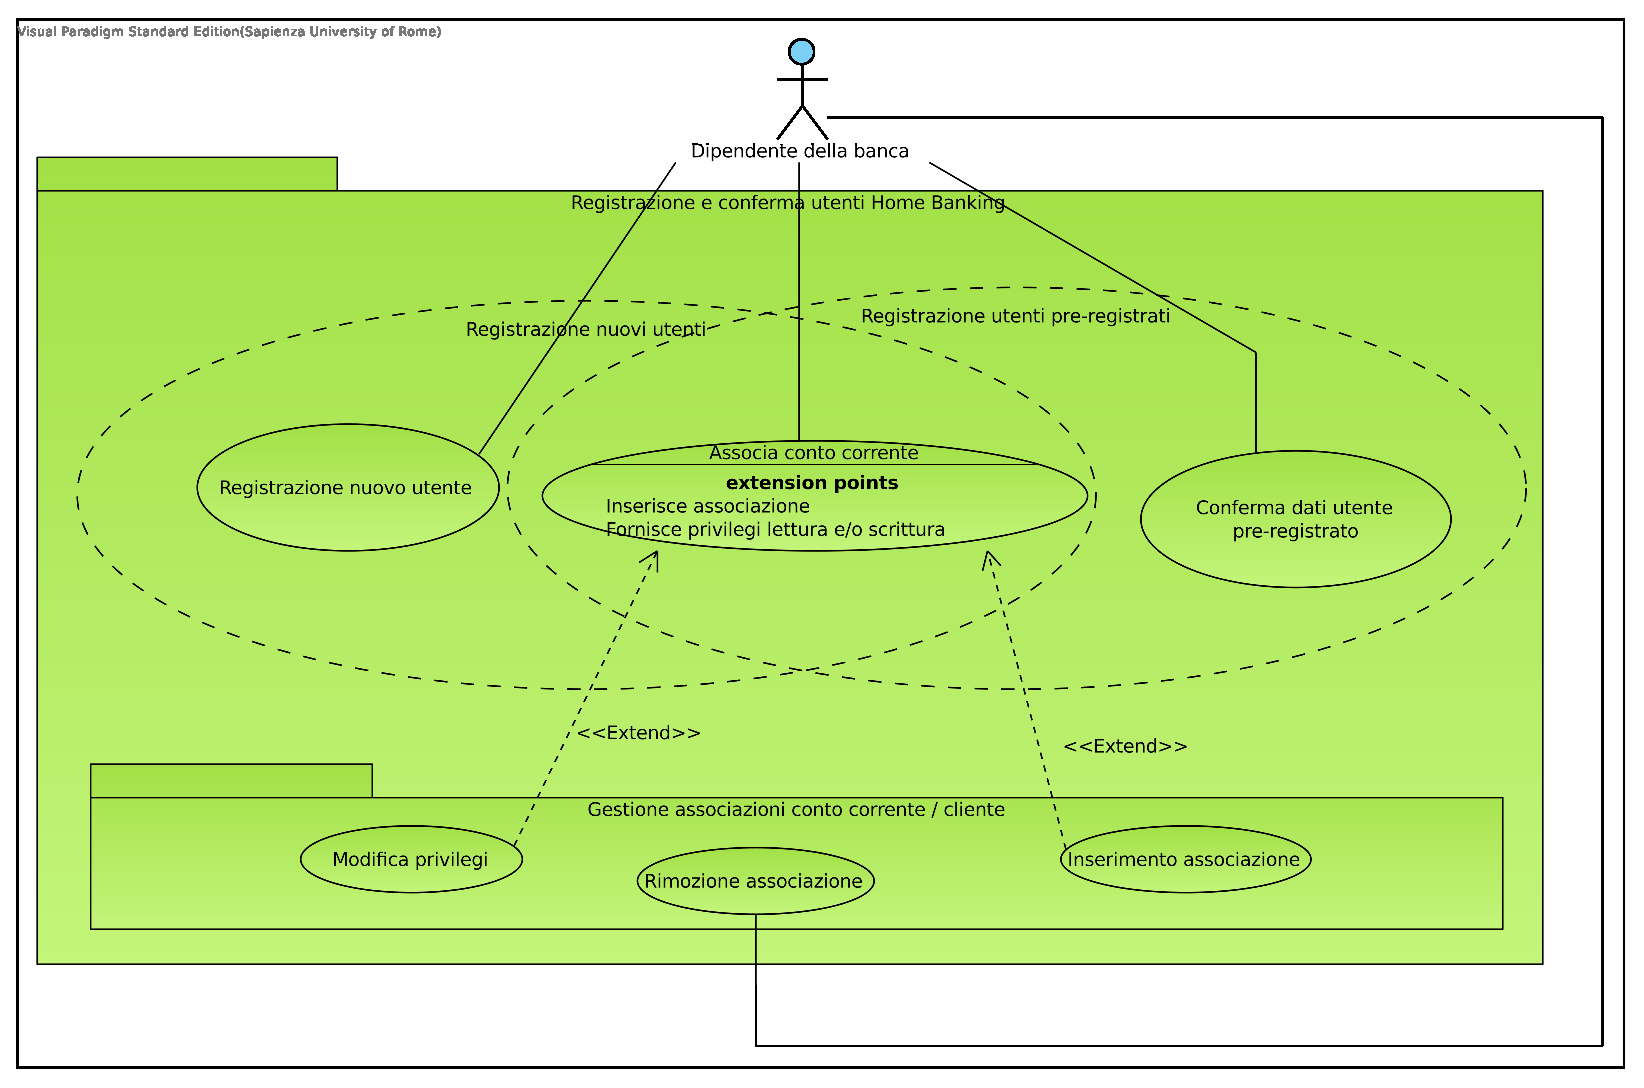
\includegraphics[width=\textwidth]{Images/use-cases/Registrazione_e_conferma_utenti_Home_Banking.eps}
	\caption{Diagramma degli use case per la registrazione e gestione degli utenti da parte dell'amministrazione della banca.}
	\label{fig:use-cases:amministrazione:gestione-utenti}
\end{figure*}

\begin{figure*}
	\centering
	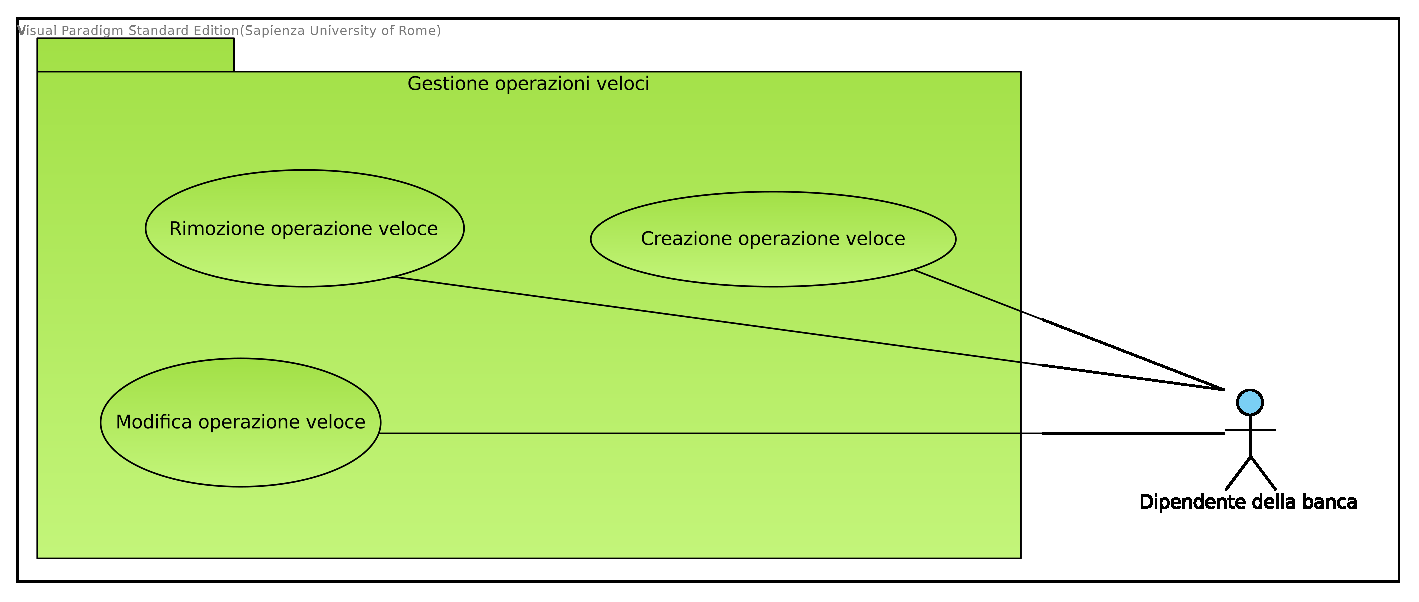
\includegraphics[width=\textwidth]{Images/use-cases/Gestione_operazioni_veloci.eps}
	\caption{Diagramma degli use case per la gestione delle operazioni veloci.}
	\label{fig:use-cases:amministrazione:gestione-operazioni-veloci}
\end{figure*}

\begin{figure*}
	\centering
	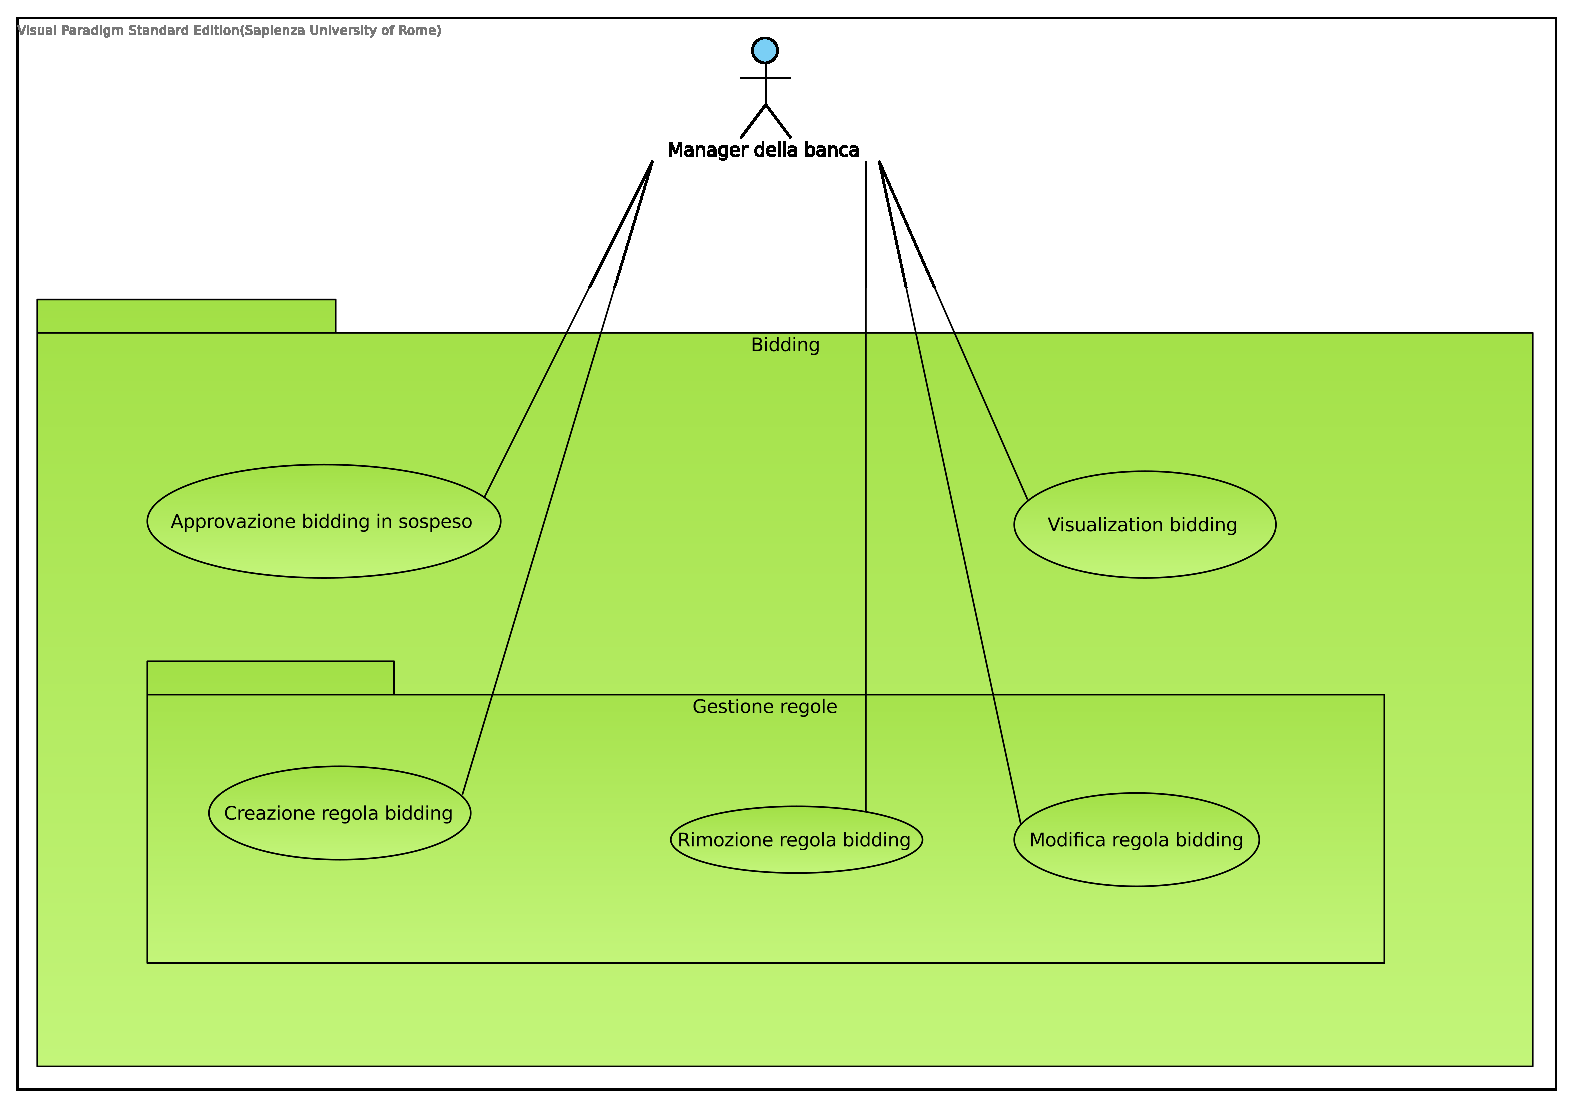
\includegraphics[width=\textwidth]{Images/use-cases/Definizione_parametri_e_approvazione_bidding.eps}
	\caption{Diagramma degli use case per la gestione delle regole di bidding.}
	\label{fig:use-cases:amministrazione:gestione-bidding}
\end{figure*}
